
\chapter{AI for Law vs. Law on AI}

Different subjects can be covered on this course:
\begin{itemize}
    \item \textbf{AI for the Law}: AI can be used to improve the efficiency of the legal system. For example, AI can be used to predict the outcome of a trial, to help lawyers in their research, to help judges in their decisions, etc.
    \item \textbf{AI as Law}: AI can be used to create new laws, for example, to regulate the use of AI. In fact, algorithms sometimes can nudge, control and repress social behaviors, in a way more effective than traditional legal tools.
    Social measurements tend to give rise to self-fulfilling prophecies and anchoring effects, like
    \begin{enumerate}
        \item \texttt{Hawthorne Effect}
        
        The Hawthorne effect is a type of reactivity in which individuals modify an aspect of their behavior in response to their awareness of being observed.
        \item \texttt{Cambpell's Law}
        
        The more any quantitative social indicator is used for social decision-making, the more subject it will be to corruption pressures and the more apt it will be to distort and corrupt the social processes it is intended to monitor.
        \item \texttt{Goodhart's Law}
        
        When a measure becomes a target, it ceases to be a good measure.
    \end{enumerate}
    \begin{figure}[H]
        \centering
        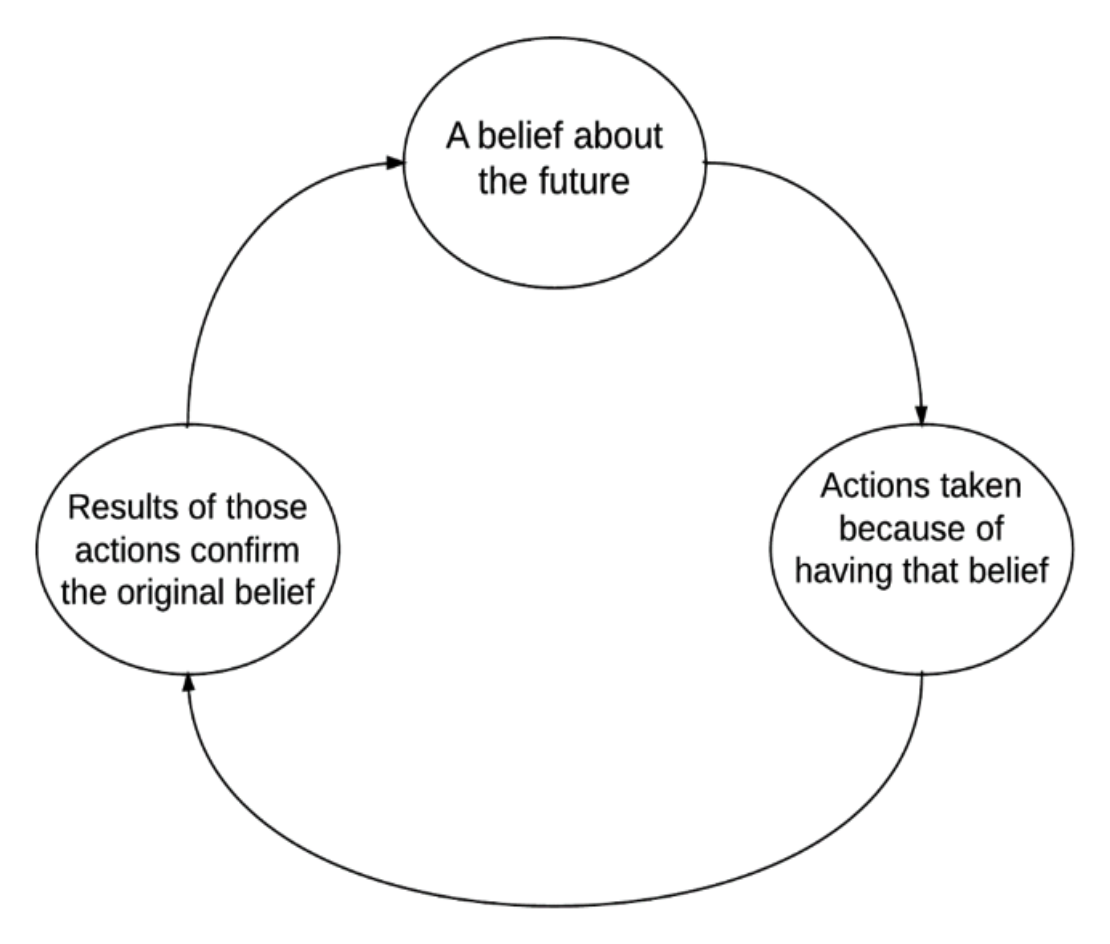
\includegraphics[width=0.5\textwidth]{assets/fig1.png}
        \caption{AI as Law}
        \label{fig:ai-law}
    \end{figure}
    \item \textbf{Law for AI}: AI can be used to regulate the use of AI. For example, AI can be used to prevent the use of AI for illegal purposes, to prevent the use of AI for discrimination, etc. 
    When we talk about regulating AI, we talk about a nnumber of different legal and geographical areas. For example, the European Union has a different approach to AI than the United States. In the absence of harmonized law, AI regulation is in principle national. This means that every single state has its own regulation and laws applying to AI.
    \begin{figure}[H]
        \centering
        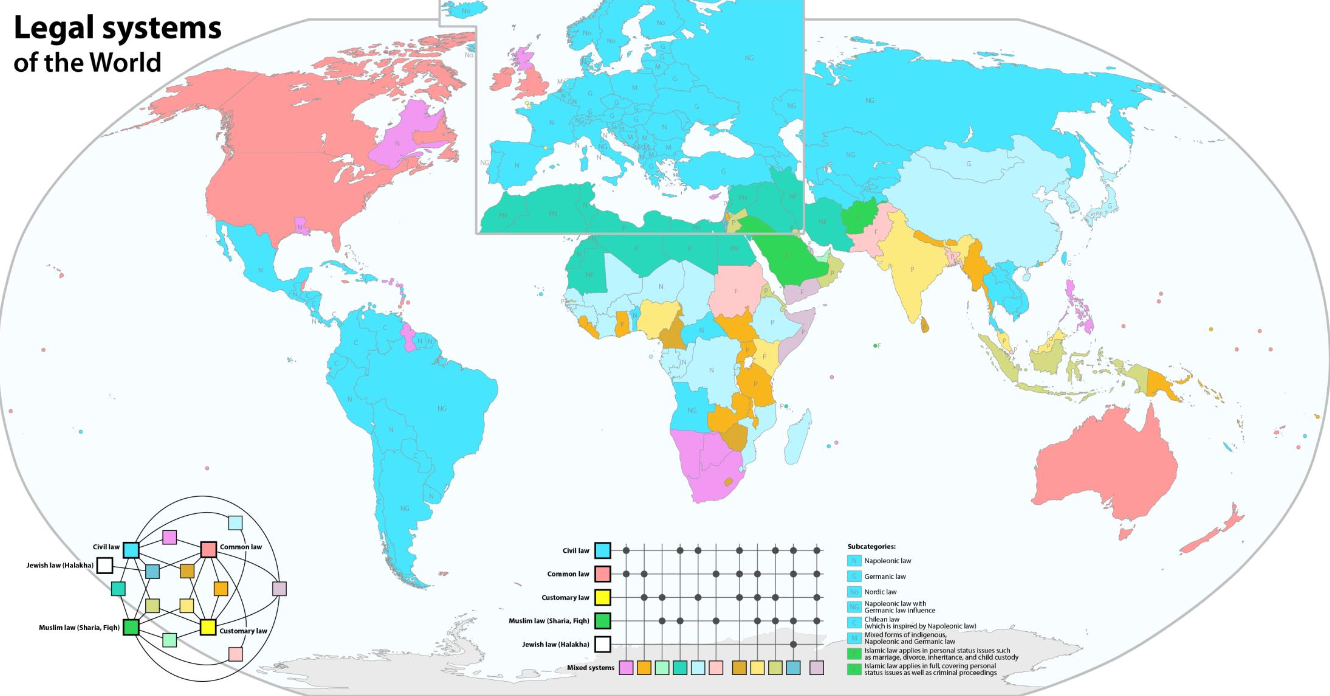
\includegraphics[width=0.9\textwidth]{assets/fig2.png}
        \caption{Law for AI}
        \label{fig:law-ai}
    \end{figure}
\end{itemize}

\begin{table}[H]
\centering
\begin{tabular}{p{0.5\textwidth} p{0.5\textwidth}}
\toprule
\textbf{EU} & \textbf{US} \\
\midrule
\textbf{Privacy as human dignity} & \textbf{Privacy as Liberty} \\
Privacy as a right for nobles, then levelled up to people & Privacy as a right against unlawful searches and seizures \\
Strict enforcement of privacy rules against any data controller & Limitations on government's power Reliance on the free market \\
\bottomrule
\end{tabular}
\caption{EU vs. US on Privacy Law}
\label{tab:privacy_law}
\end{table}



